\chapter*{Sommario} % senza numerazione
\label{sommario}

\addcontentsline{toc}{chapter}{Sommario} % da aggiungere comunque all'indice
\vspace{5mm}

\emph{Segue una breve introduzione sul progetto sviluppato e sulla sua reimplementazione secondo quanto introdotto precedentemente.} \vspace{5mm}

\section{Il progetto}\vspace{5mm}

Un ente pubblico come può essere un piccolo comune storico italiano necessita di una comunicazione efficiente e diretta con i propri visitatori. Nel caso di Open Air Museum, si trattava di un progetto nato per guidare e indirizzare i turisti del Comune in questione all’interno della loro città, storicamente e culturalmente ricca, con una guida virtuale che avrebbe potuto sostituire una persona fisica come guida turistica della zona. Data la grande varietà linguistica dei possibili utenti il prodotto è stato sviluppato multilingue.

\section{Open Air Museum}\vspace{5mm}

Il progetto Open Air Museum è stato sviluppato da me e i miei colleghi del reparto di Sviluppo Software di Farnedi ICT, azienda informatica di Cesena. Consiste di un’applicazione mobile per dispositivi iOS, di una seconda applicazione per dispositivi Android e di un software in Filemaker per il caricamento dei contenuti. In particolare io mi sono occupato dello sviluppo dell’applicazione mobile per iOs in Swift 3 e dell’applicativo lato server in NodeJs. \vspace{5mm}

L’applicazione consiste in una guida turistica e multimediale in grado di mostrare ai suoi utenti una serie di punti di interesse collegati da percorsi preimpostati. Ogni punto dispone di un pacchetto multimediale di audio e immagini oltre ad una descrizione, un nome e delle informazioni tutte gestibili e configurabili in oltre 160 lingue. Tali punti possono essere navigati attraverso l’interfaccia grafica degli applicativi per smartphone - sfruttando la geolocalizzazione del dispositivo - oppure attraverso la modalità Esplora dell’applicazione. Quest'ultima permette, una volta attivata, di essere notificati automaticamente sulla presenza di punti di interesse nella zona circostante, dando la possibilità, o meno, all’utente di richiedere informazioni aggiuntive. Quest’ultima features è stata implementata sfruttando la tecnologia Beacon e Bluetooth 4.0, che permette al dispositivo di percepire l’ingresso in una specifica area, marcata da un piccolo radiofaro bluetooth, il quale marca di fatto un determinato punto di interesse. La metodologia con cui viene identificata una zona rispetto ad un altra è usando la firma del Beacon e cioè attraverso i suoi tre parametri identificativi, UUID, major e minor. Il primo è una stringa alfanumerica a 128 bit che ha lo scopo di identificare un gruppo di Beacon, ad esempio l’insieme posizionato all’interno del comune, mentre gli ultimi due, insieme all’UUID identificano un beacon specifico. Utilizzando lo UUID per definire una Ragion di ricerca è possibile escludere da essa tutti gli altri beacon non appartenenti all’applicativo. Infatti tutti i beacon da noi posizionati sono contraddistinti da uno specifico UUID mentre differiscono per major e minor, in modo da identificarli singolarmente. Un ulteriore metodo per gestire la “scoperta” di beacon in una regione è quello di verificarne la distanza dal telefono, così facendo si possono scartare i beacon più lontani e notificare all’utente solamente quelli più prossimi, questo è fondamentale dato che vi sono delle zone della città molto “dense” di punti di interesse e una semplice ricerca non basterebbe a definire la prossimità di un utente a un punto rispetto ad un altro; questa features ha aiutato a realizzare una localizzazione più precisa e risultando in un’esperienza d’uso migliore.\vspace{5mm}

	Attraverso l’applicativo in Filemaker, esposto tramite un’interfaccia web, i dipendenti del Comune potevano gestire l’inserimento dei punti e dei percorsi compresi di media e testi relativi. \vspace{5mm}
La visualizzazione dei punti avviene attraverso due schermate, la prima è una lista che gli mostra tutti in ordine casuale e vi è la possibilità di navigare ad una schermata più dettagliata dove vi sono le informazioni del punto selezionato ed è possibile riprodurre i contenuti multimediali associati ad esso. La seconda mostra l'elenco di tutti i percorsi disponibili, dando la possibilità, una volta selezionato, di vedere nel dettaglio di quali punti è composto e in che ordine visitarli.
	
\vspace{5mm}La parte server, invece, espone delle Rest Api che consumate forniscono sia i dati sopracitati che un servizio di autenticazione mediante Json Web Token. Questo applicativo è stato sviluppato senza l’ausilio di framework esterni per il routing o per la gestione dell’autenticazione o la generazione dei token di sessione. Node Js è stato scelto in questo caso per la sua efficienza nelle operazioni di I/O rispetto ad una tecnologia più canonica come PHP o Java, vista la grande quantità e la tipologia di file da servire. Implementando un I/O non bloccante nel caso di invio di file di medie dimensioni come audio o immagini questo risulta nel riuscire a servire più client contemporaneamente utilizzando meno risorse \cite{BlockingVsNonBlocking} \vspace{5mm}

\begin{figure}[h]
\centering
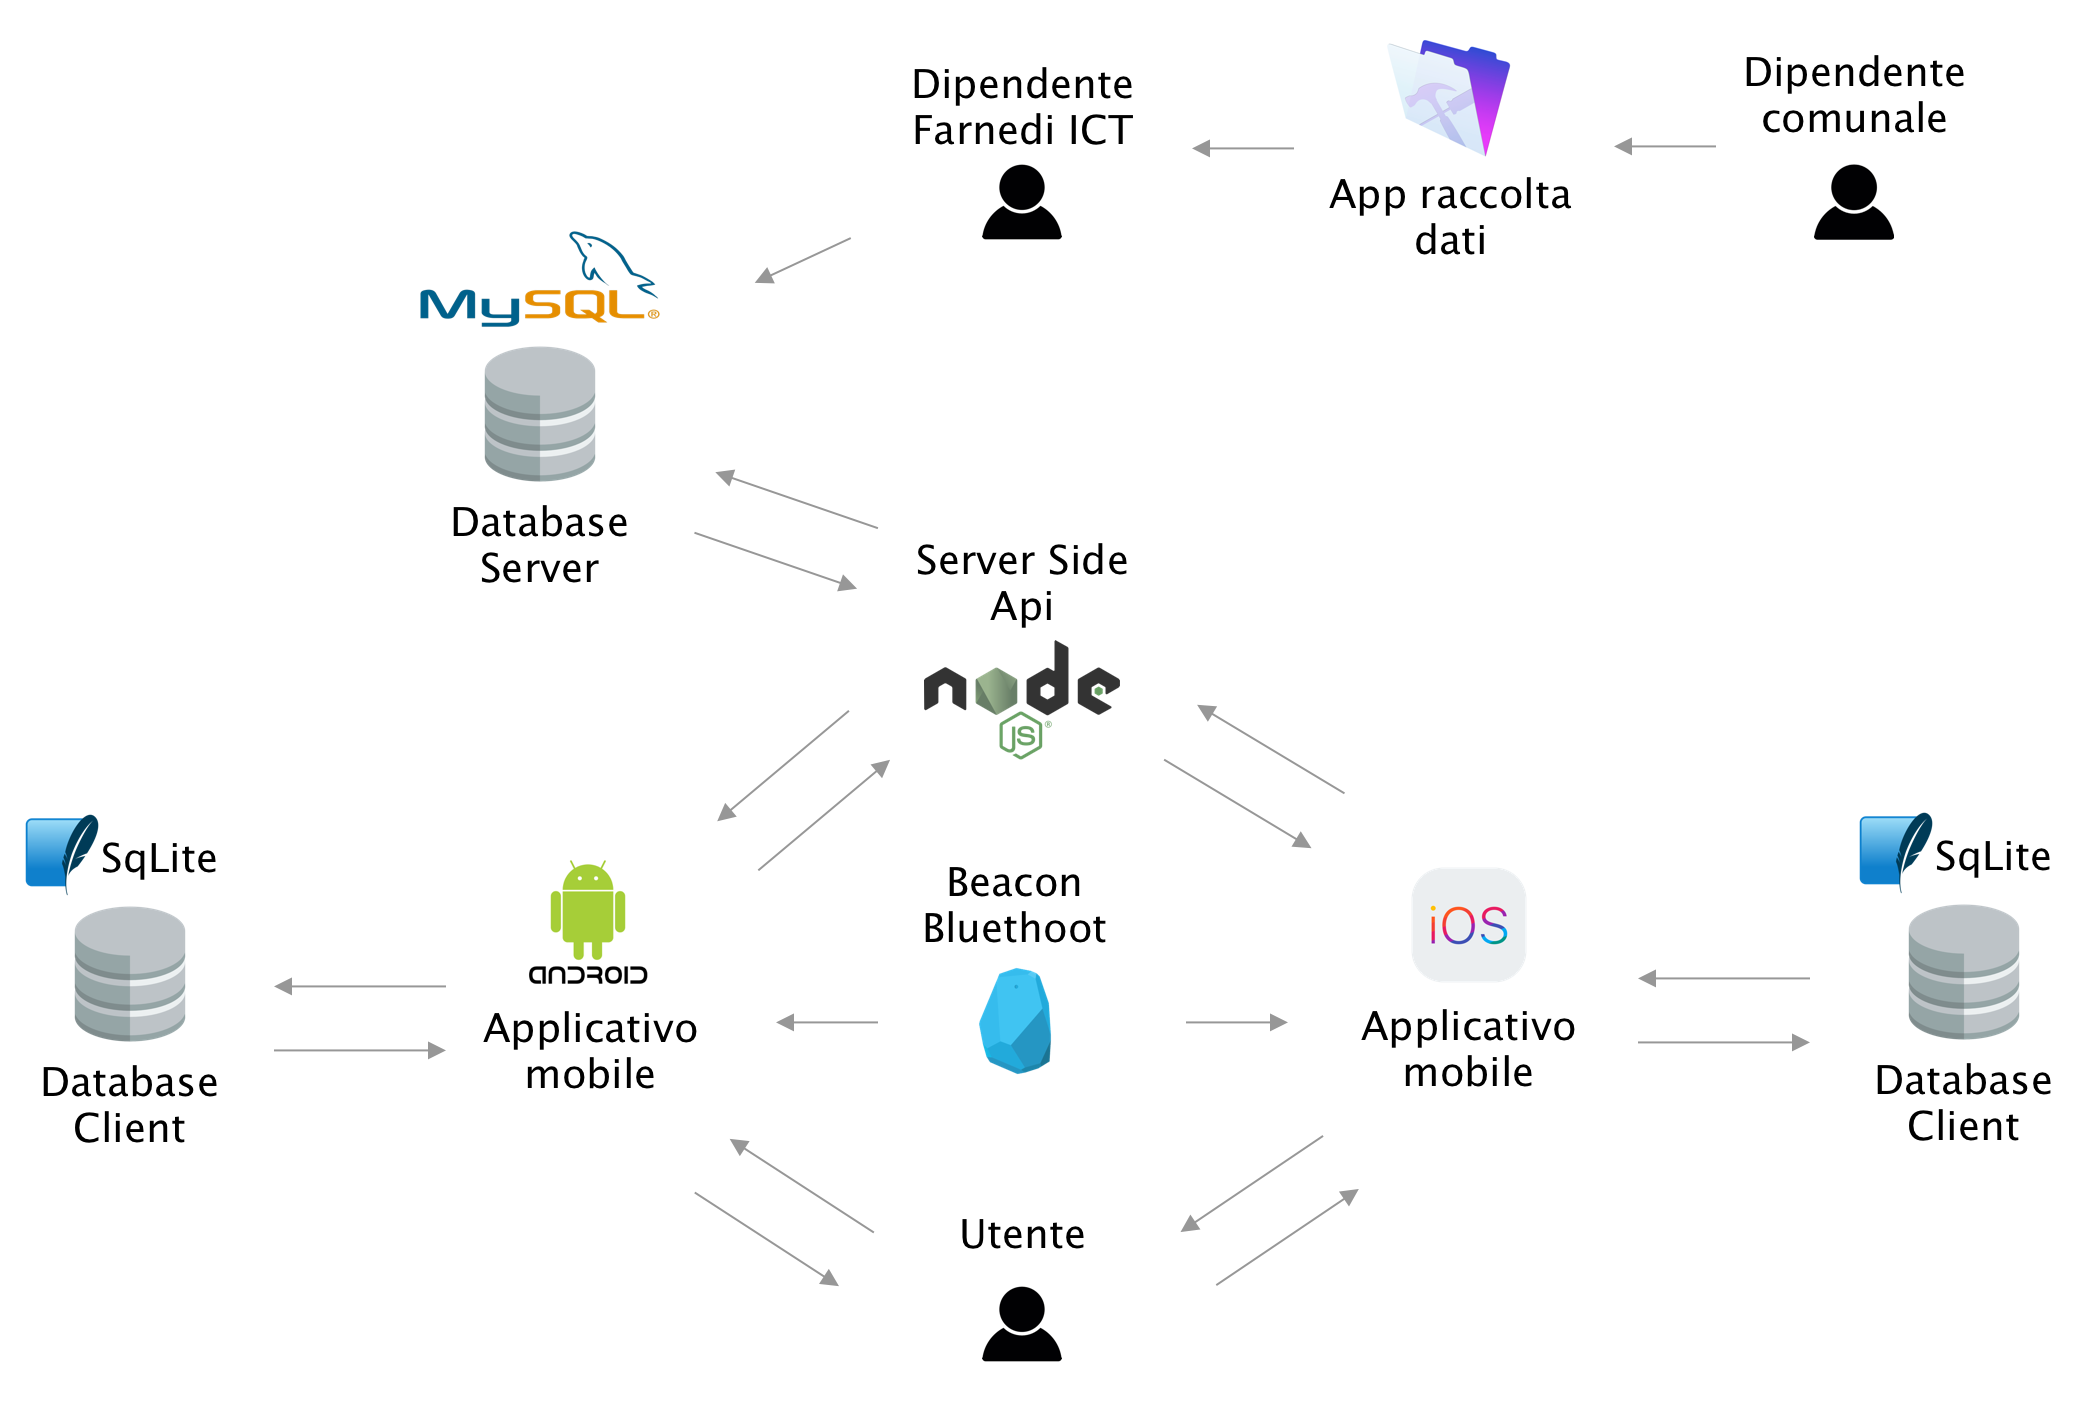
\includegraphics[width=0.9\textwidth]{images/SchemaOpenAirMuseum.png}
\caption{Schema logico dello stack di Open Air Museum}
\end{figure}

\section{Obiettivo e struttura della tesi}\vspace{5mm}

	L’obiettivo di questa tesi è dimostrare che è possibile, per un prodotto completo di questo tipo, riscrivere la totalità degli applicativi che lo compongono in Javascript e che questo sia un vantaggio sia dal punto di vista dei costi di gestione che dell’effettiva manutenibilità del progetto, mantenendo le medesime funzionalità e senza alterare la qualità del prodotto. Inoltre valuterò l’efficacia di adottare uno stack Javascript soppesando i costi di sviluppo e il peso tecnologico utilizzando come metro di paragone le ore impiegate nello sviluppo dello stack “tradizionale” rispetto a quello Javascript.
Il capitolo 2 descrive le tecnologie disponibili attualmente sul mercato candidate a sostituire quelle impiegate nella versione precedente dell’applicativo. Il capitolo 3 analizza le scelte tecnologiche fatte ponendo un confronto tra le due versioni. Il capitolo 4 definisce più nel dettaglio il porting degli applicativi mobile illustrando i processi e le criticità legate a questa operazione. Il capitolo 5 descrive la possibilità di costruire un process manager per istanze del prodotto. Infine nel capitolo 6 viene eseguita un’analisi e una valutazione del lavoro svolto, con relative conclusioni. 








